\documentclass{article}


\usepackage[widepage]{repsty}
\usepackage{extarrows}


\newcommand{\Wx}{\Omega_x}
\newcommand{\Wy}{\Omega_y}
\newcommand{\yG}{\gamma G}
\newcommand{\Dx}{\Delta x}
\newcommand{\Dy}{\Delta y}




\begin{document}
	TBMT equation:
	\begin{align*}
		\Wx &= a(\yG)\cdot B_x,\\
		\Wy &= a(\yG)\cdot B_y.
	\end{align*}
	
	\paragraph{Argument 1. [$\gamma \equiv \gamma_{eff}$]:}
	Let $\vec{B}\cdot\vec{B}' = BB'\cos\theta, \theta\neq0$. (Fig.~\ref{fig:Arg1}.)
	
	$\gamma = \gamma' \land \Wy = \Wy' \xLongrightarrow{\text{TBMT}} B_y = B_y' \xLongrightarrow{\theta\neq0} B_x\neq B_x'$.
	
	\begin{figure}[h]\centering
			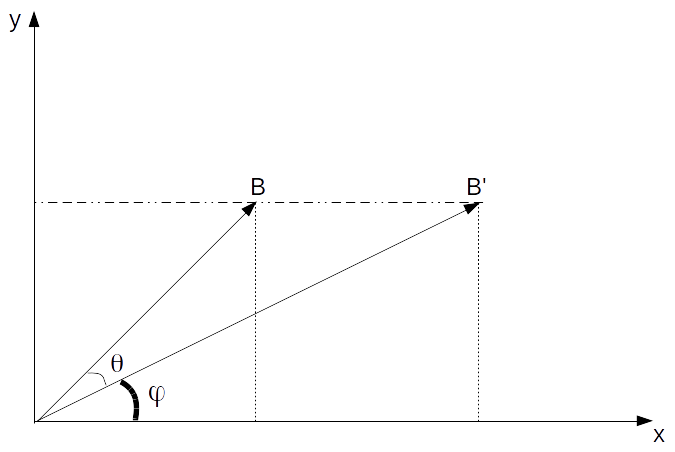
\includegraphics[scale=.5]{img/Field}
			\caption{Argument 1 illustration.\label{fig:Arg1}}
	\end{figure}
	
	\begin{align*}
		\Wx' &= a \vec{B}'\cdot\hat{x} = a B' \cos\phi = B_y \tan\phi,\\
		\Wx &= a \vec{B}\cdot\hat{x} = a B\cos(\theta+\phi) = B_y \tan(\theta+\phi),\\
		\frac{\Wx}{\Wx'} &= \frac{\tan(\theta+\phi)}{\tan\phi}.
	\end{align*}
	
	\paragraph{Argument 2. [$\gamma \equiv \gamma_s$]:}
	
	
	\[
		\gamma_{eff} = f(\gamma_s,\Dx,\Dy).
	\]
	
	\begin{figure}[h]
		\centering
		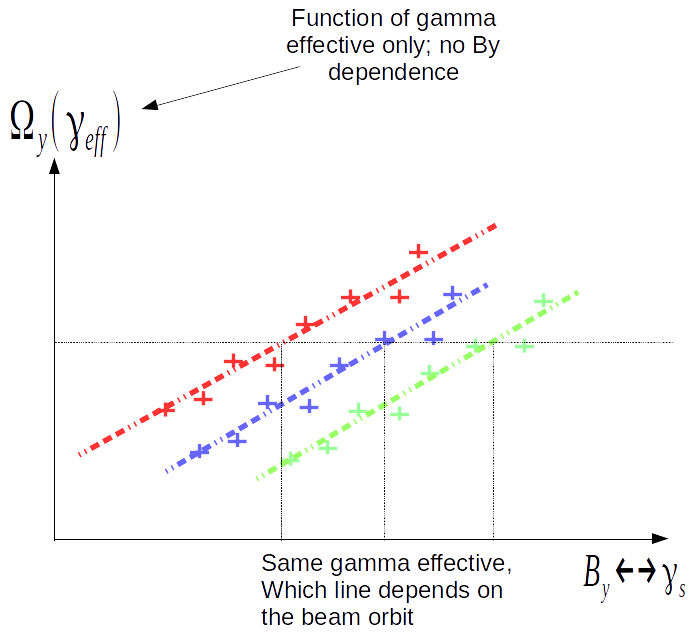
\includegraphics[scale=.5]{img/Argument2}
	\end{figure}
	
%	\begin{align*}
%		\gamma &= (1-\beta^2)^{-\sfrac12}, \\
%		\beta &= \frac{R}{mc} B_y = b(R)\cdot B_y,\\
%		\Wy &= a\bkt{\bkt*{1-b(R)^2B_y^2}G} \cdot B_y,\\
%		\Wy' &=a\bkt{\bkt*{1-b(R')^2B_y'^2}}\cdot B_y'
%	\end{align*}
	
	
\end{document}